This open-source project (github.com/clawoflight/aursec) was done by three people: Two students who implemented the tool and their supervisor. This required considerable communication and time management. 

\subsubsection*{timeline}
From the timeline (Figure \ref{fig:timeline}) can be derived that this project was realized in less then 9 months. The real worktime exposure ratio of the three main-task (reading, programming and writing) differs extremely from the visualized one. In reality we read 50\%, programmed 40\% and wrote 10\% of the worktime.
It is also visible that we didn't manage to complete three milestones in time. This was caused by different circumstances, but we managed to complete the hole project in time cause we adjusted our planing every few weeks.

\begin{figure}[!htb]
	\centering
		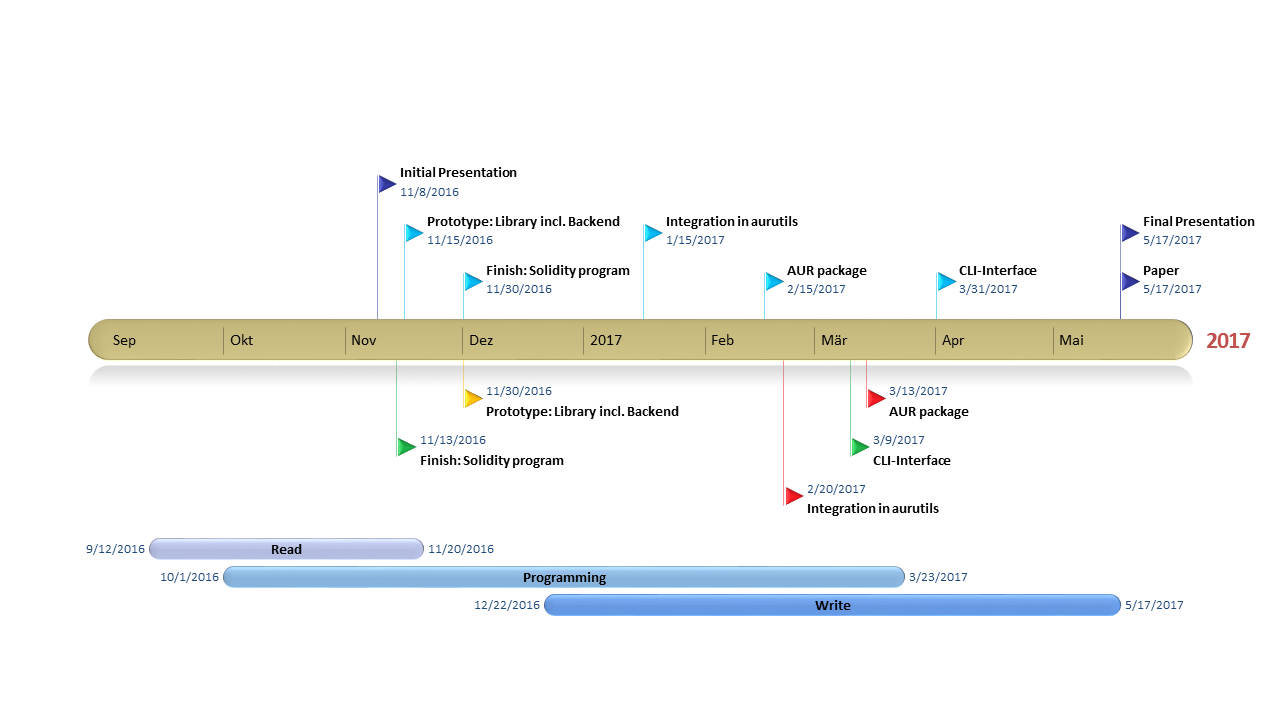
\includegraphics[width=0.7\paperwidth]{timeline}
	\caption{Timeline}
	\label{fig:timeline}
\end{figure}
